\chapter{Sheet strain}\label{sec:sheet_stretch}

\cref{fig:tetrahedron_strain} and~\cref{fig:honeycomb_strain} shows the sheet-substrate system during a strain simulation. For these simulaitons we used a slower strain speed of $\SI{0.001}{ps^{-1}} = \SI{0.1}{\%ps^{-1}}$ in order to get more clean figures. However, this did not make any noticeable changes to the development of the contact-strain curves. Otherwise, the default values from~\cref{tab:final_param} are followed.


\newpage



\begin{figure}[H]
    \centering
    \begin{subfigure}[b]{0.49\textwidth}
        \centering
        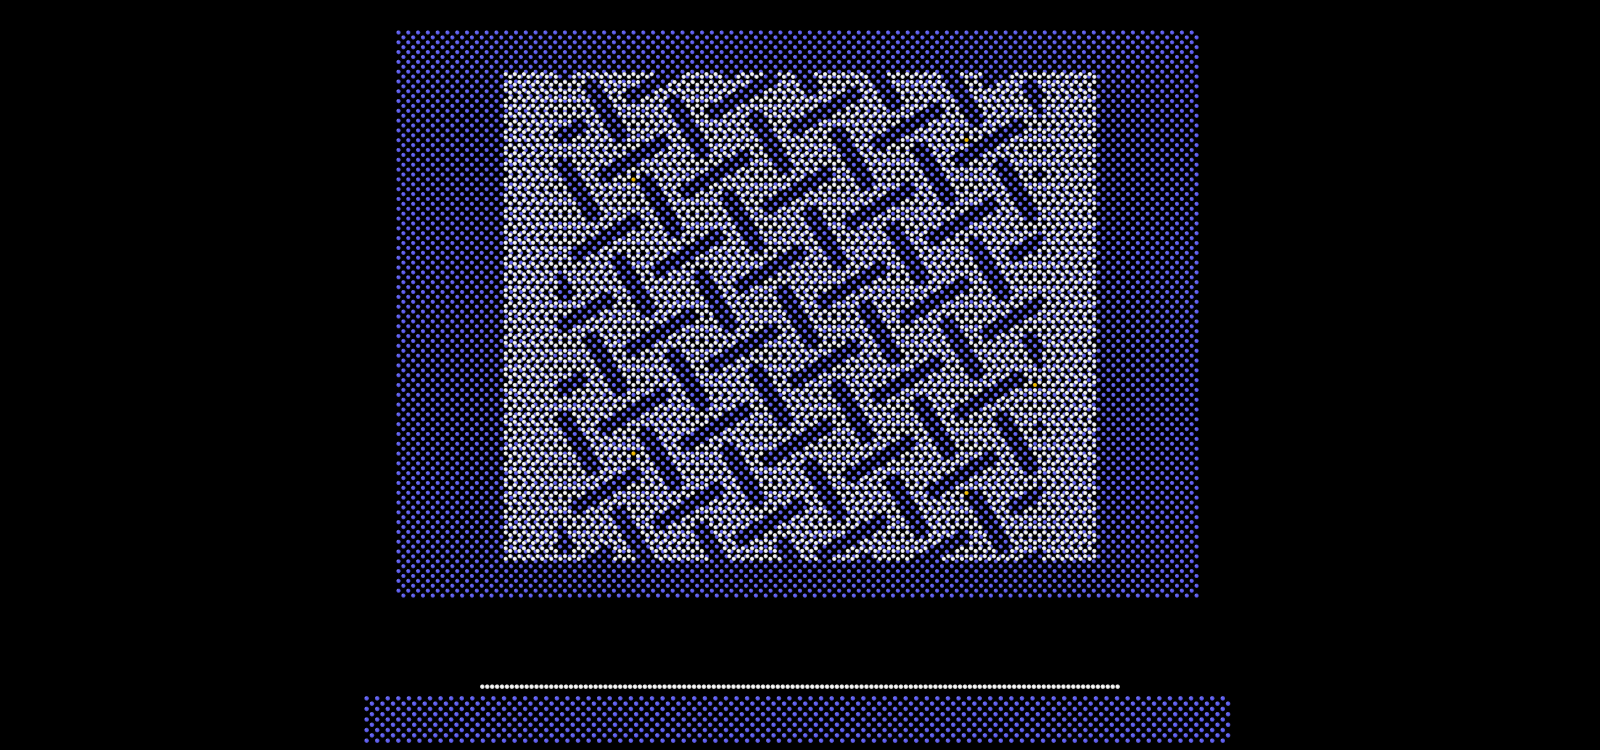
\includegraphics[width=\textwidth]{figures/baseline/contact_vs_stretch/popup/pop_stretch0000.png}
        \caption{Strain = 0.00}
        % \label{fig:}
    \end{subfigure}
    \hfill
    \begin{subfigure}[b]{0.49\textwidth}
        \centering
        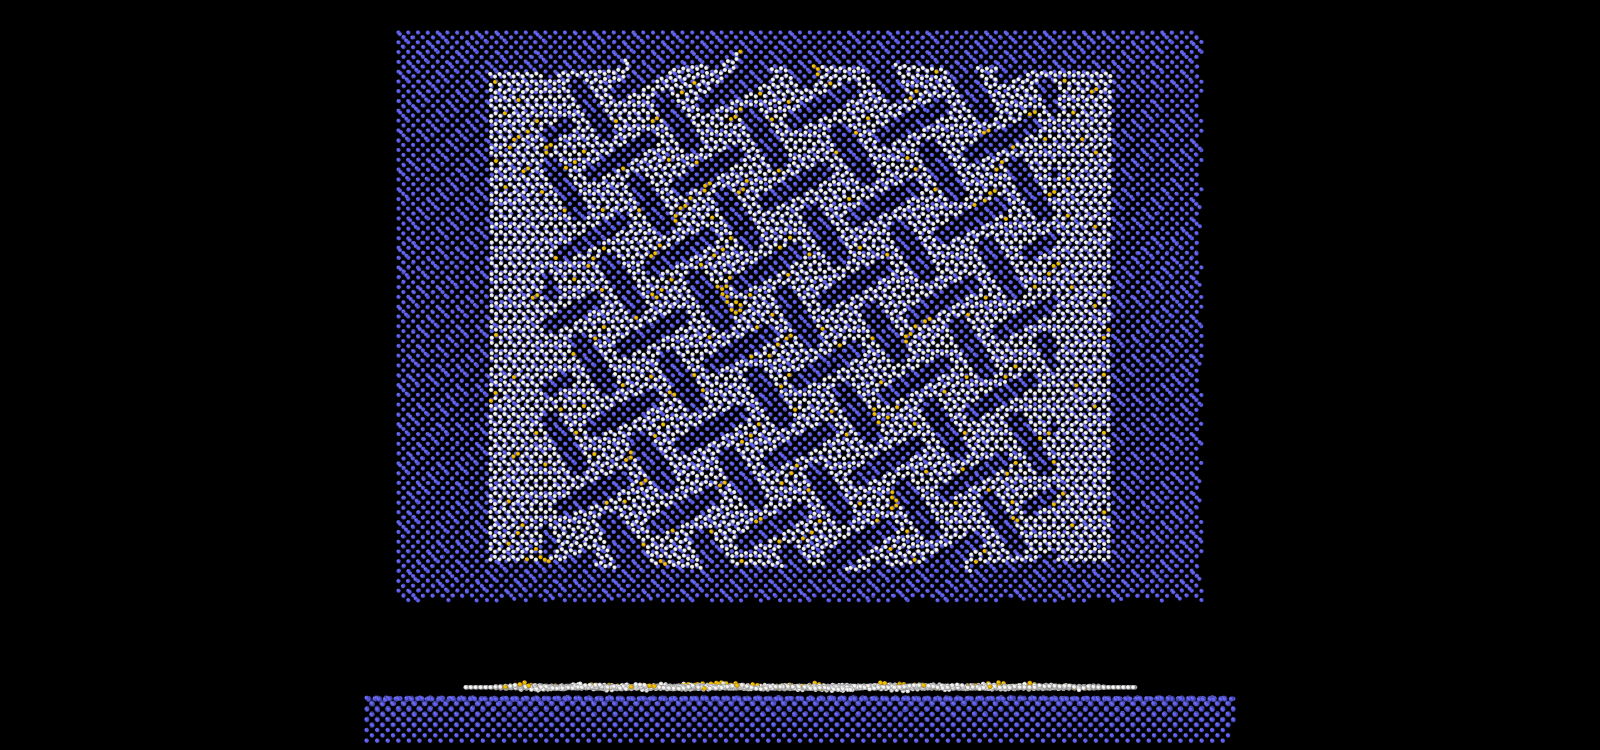
\includegraphics[width=\textwidth]{figures/baseline/contact_vs_stretch/popup/pop_stretch0006.png}
        \caption{Strain = 0.06}
        % \label{fig:}
    \end{subfigure}
    \begin{subfigure}[b]{0.49\textwidth}
        \centering
        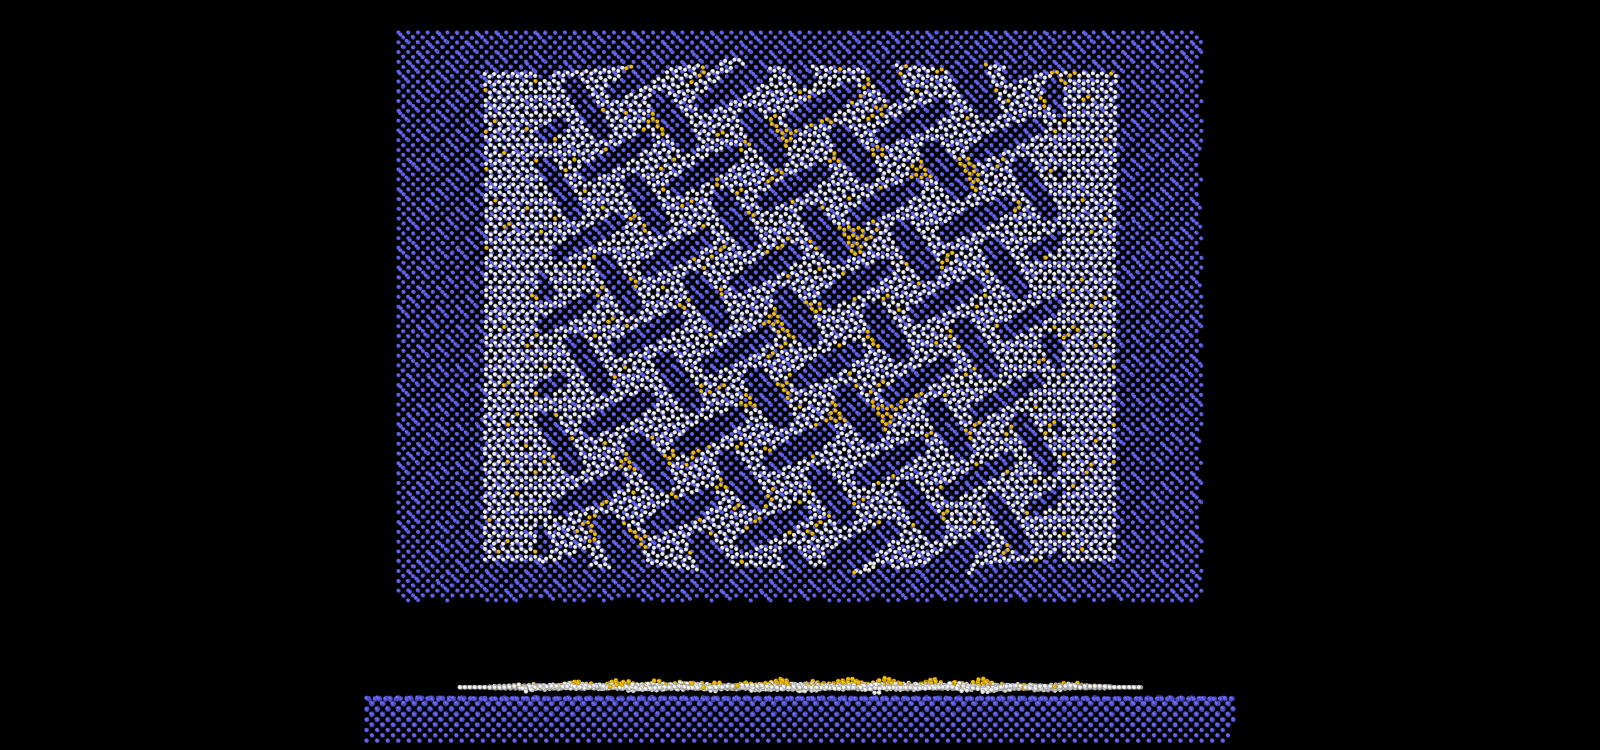
\includegraphics[width=\textwidth]{figures/baseline/contact_vs_stretch/popup/pop_stretch0008.png}
        \caption{Strain = 0.08}
        % \label{fig:}
    \end{subfigure}
    \hfill
    \begin{subfigure}[b]{0.49\textwidth}
        \centering
        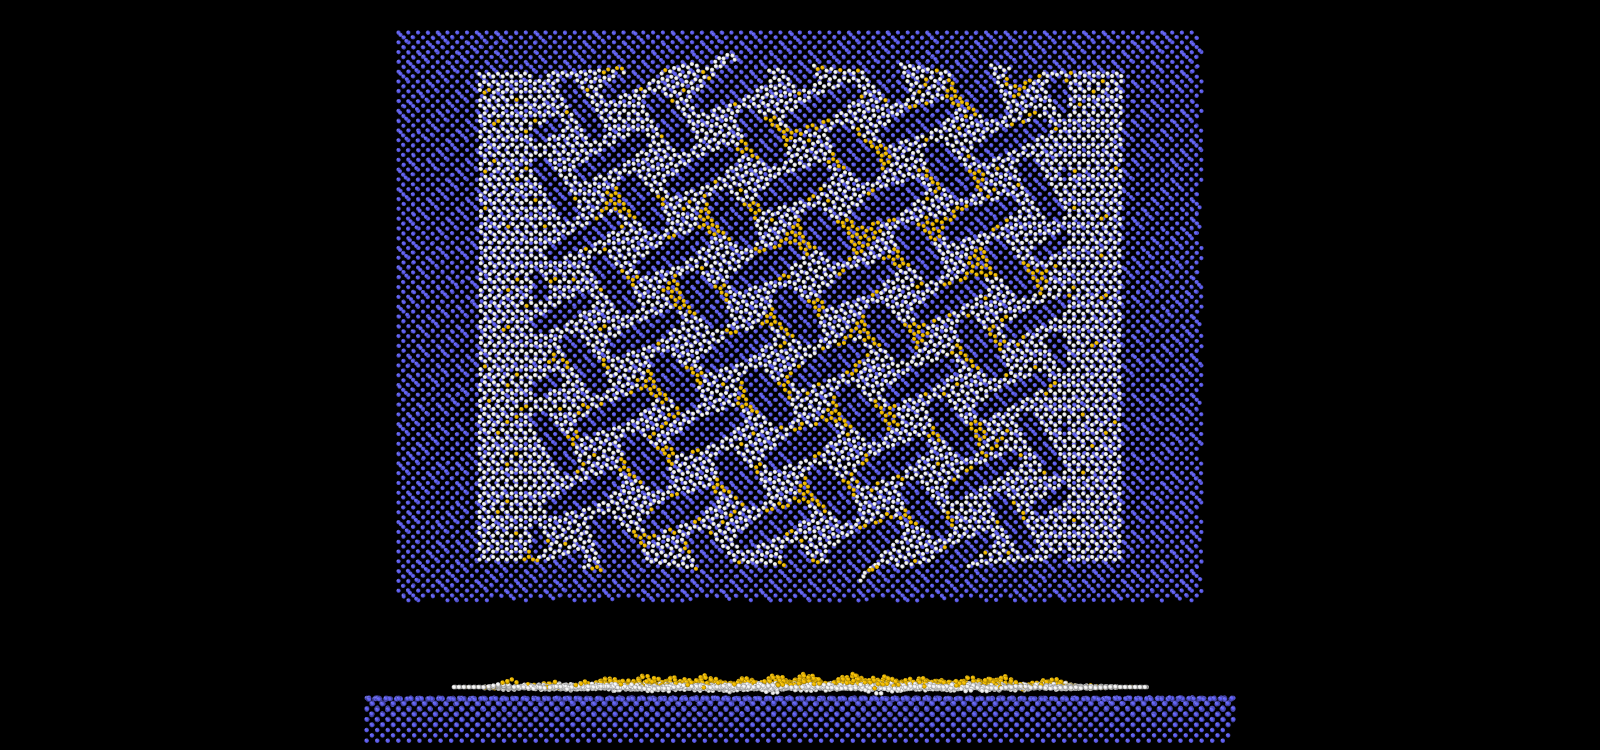
\includegraphics[width=\textwidth]{figures/baseline/contact_vs_stretch/popup/pop_stretch0010.png}
        \caption{Strain = 0.10}
        % \label{fig:}
    \end{subfigure}
    \hfill
    \begin{subfigure}[b]{0.49\textwidth}
        \centering
        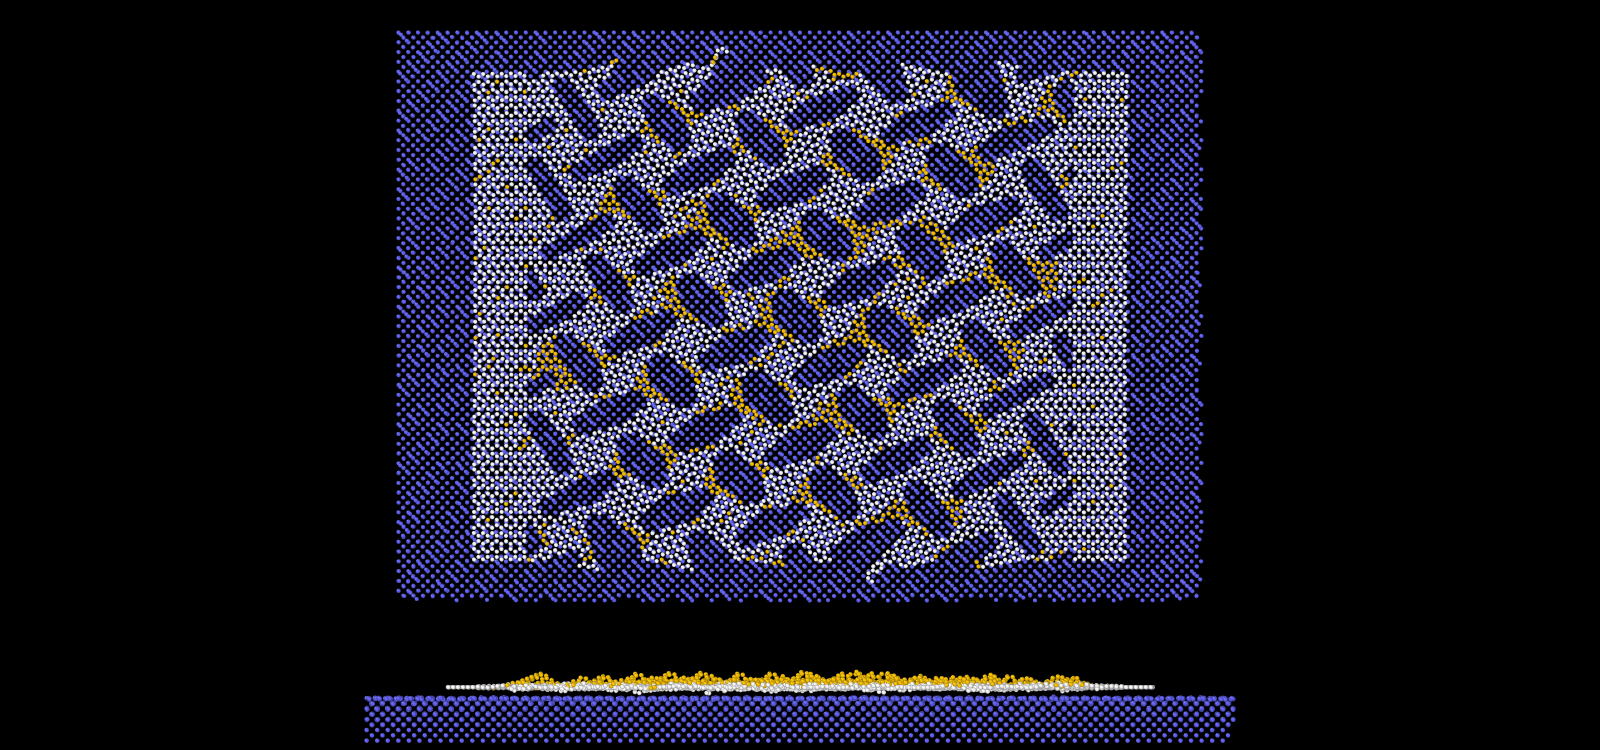
\includegraphics[width=\textwidth]{figures/baseline/contact_vs_stretch/popup/pop_stretch0012.png}
        \caption{Strain = 0.12}
        % \label{fig:}
    \end{subfigure}
    \hfill
    \begin{subfigure}[b]{0.49\textwidth}
        \centering
        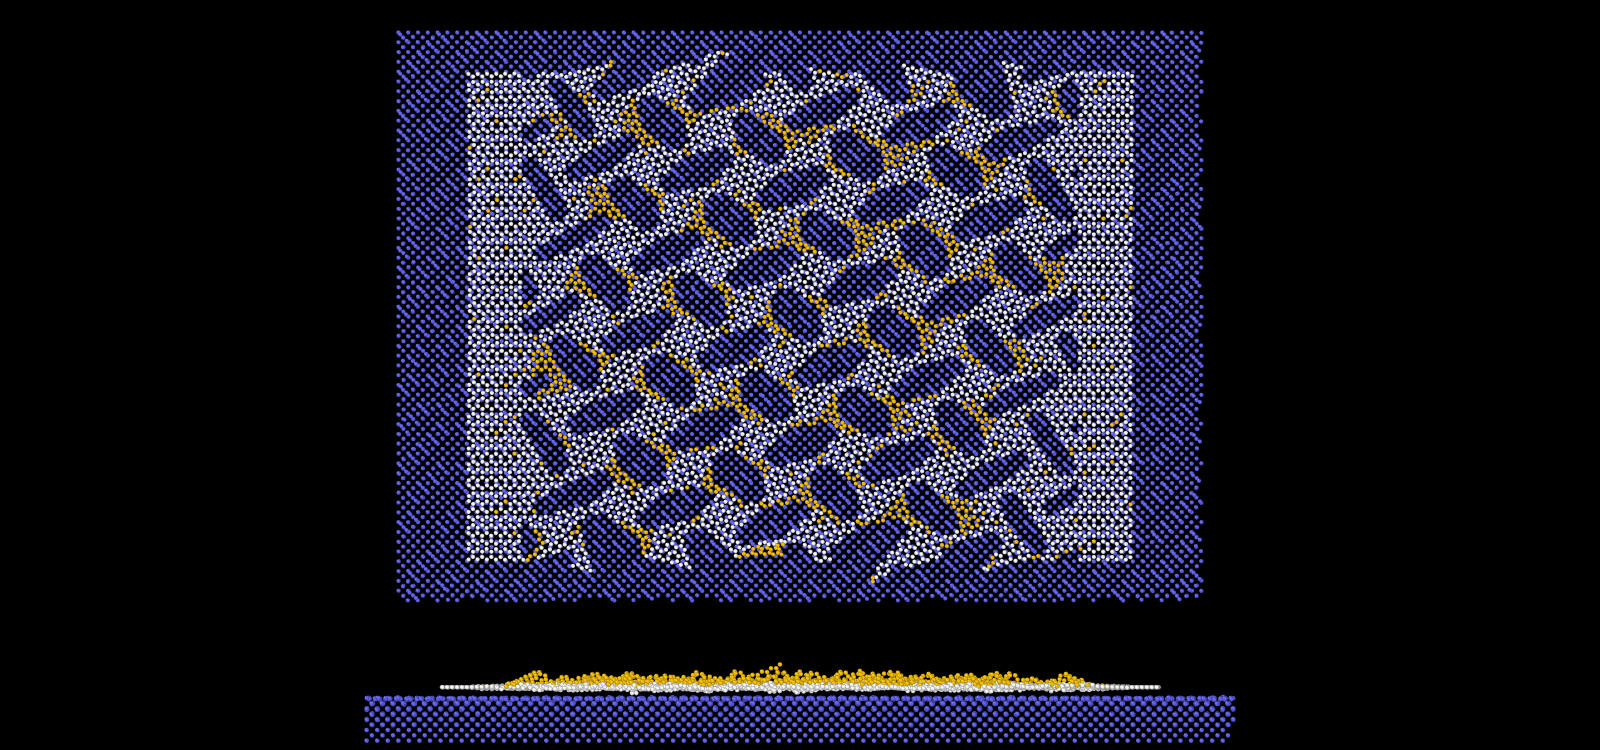
\includegraphics[width=\textwidth]{figures/baseline/contact_vs_stretch/popup/pop_stretch0014.png}
        \caption{Strain = 0.14}
        % \label{fig:}
    \end{subfigure}
    \begin{subfigure}[b]{0.49\textwidth}
        \centering
        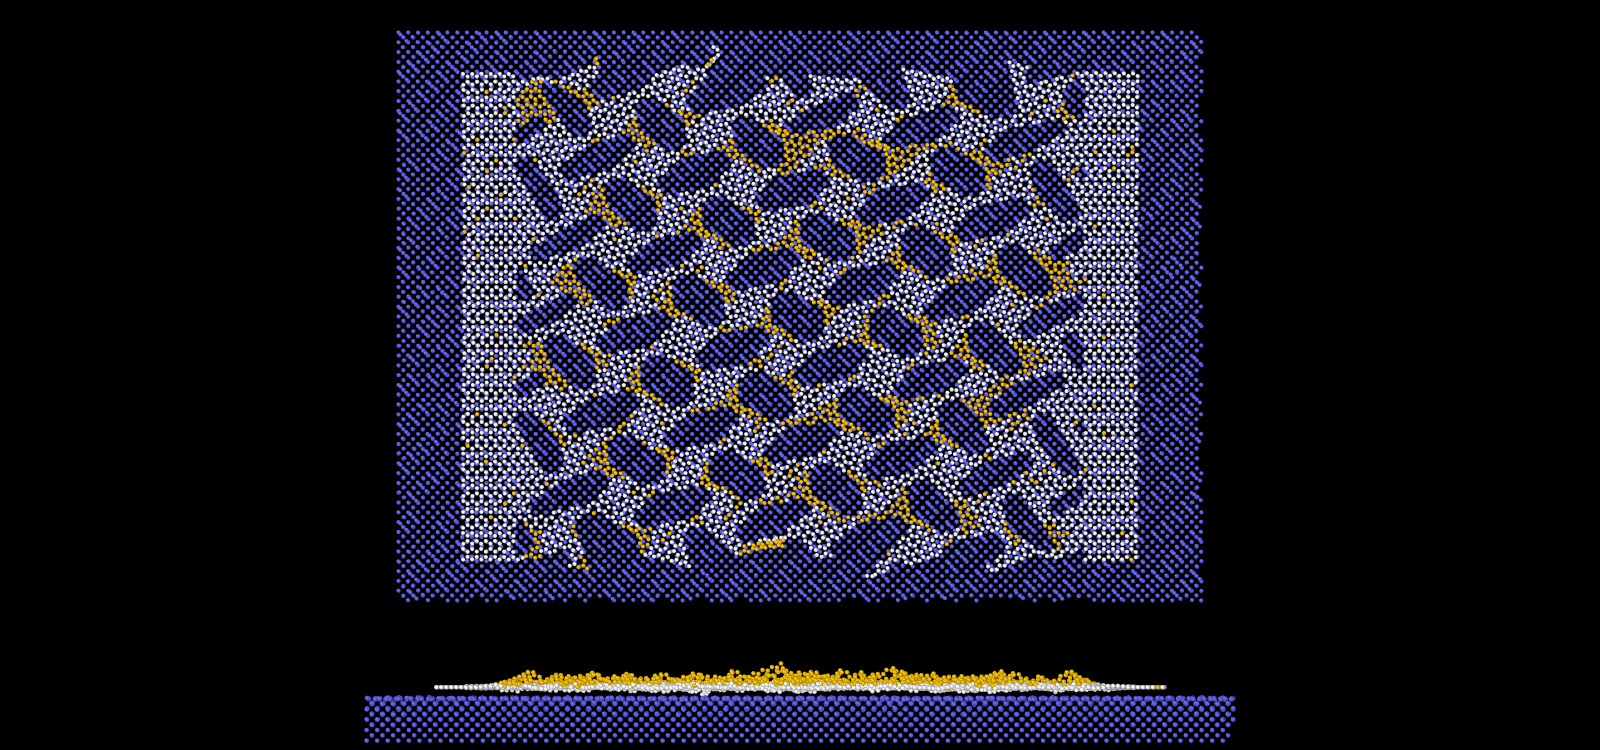
\includegraphics[width=\textwidth]{figures/baseline/contact_vs_stretch/popup/pop_stretch0016.png}
        \caption{Strain = 0.16}
        % \label{fig:}
    \end{subfigure}
    \hfill
    \begin{subfigure}[b]{0.49\textwidth}
        \centering
        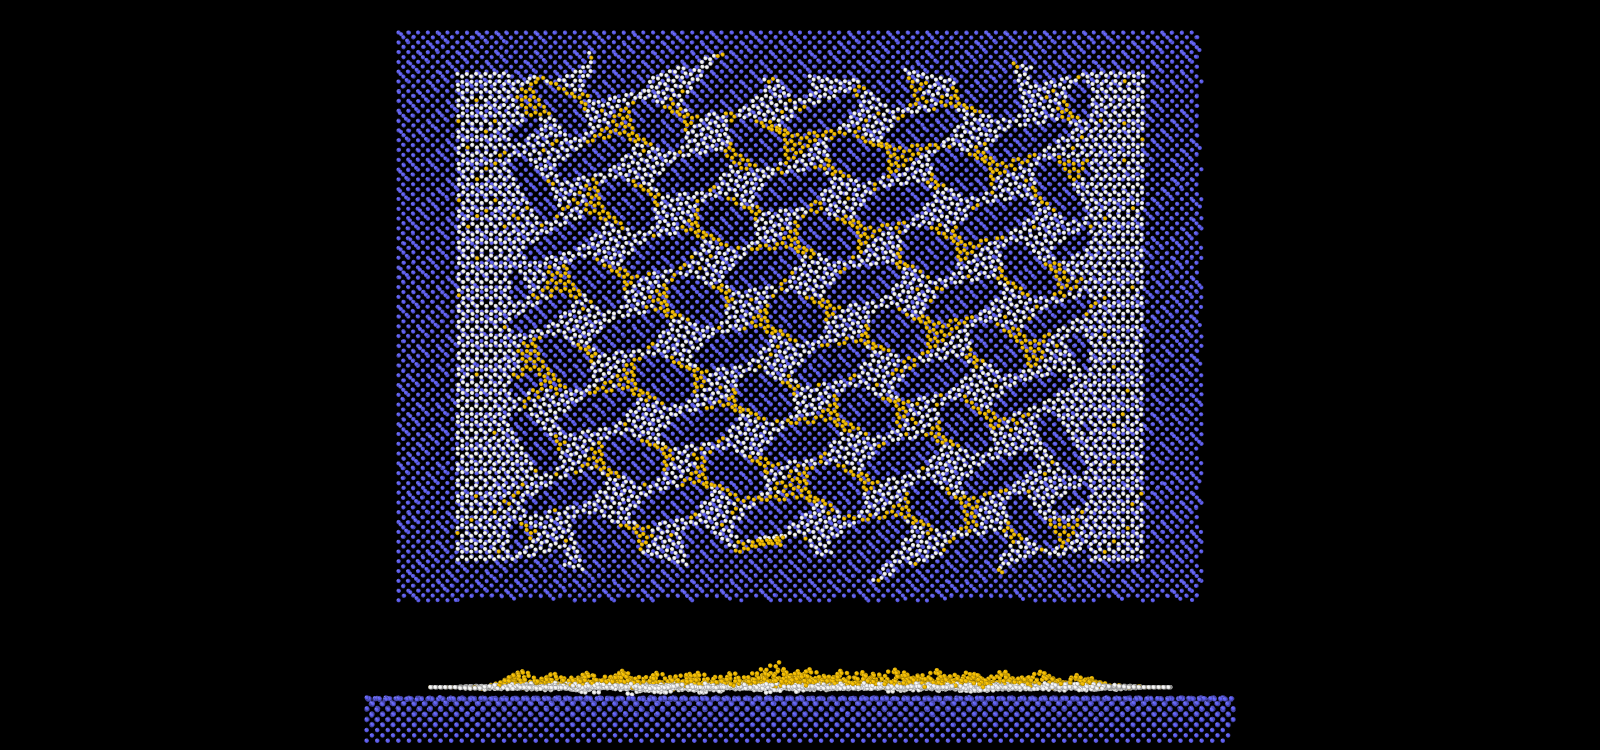
\includegraphics[width=\textwidth]{figures/baseline/contact_vs_stretch/popup/pop_stretch0018.png}
        \caption{Strain = 0.18}
        % \label{fig:}
    \end{subfigure}
    \begin{subfigure}[b]{0.49\textwidth}
        \centering
        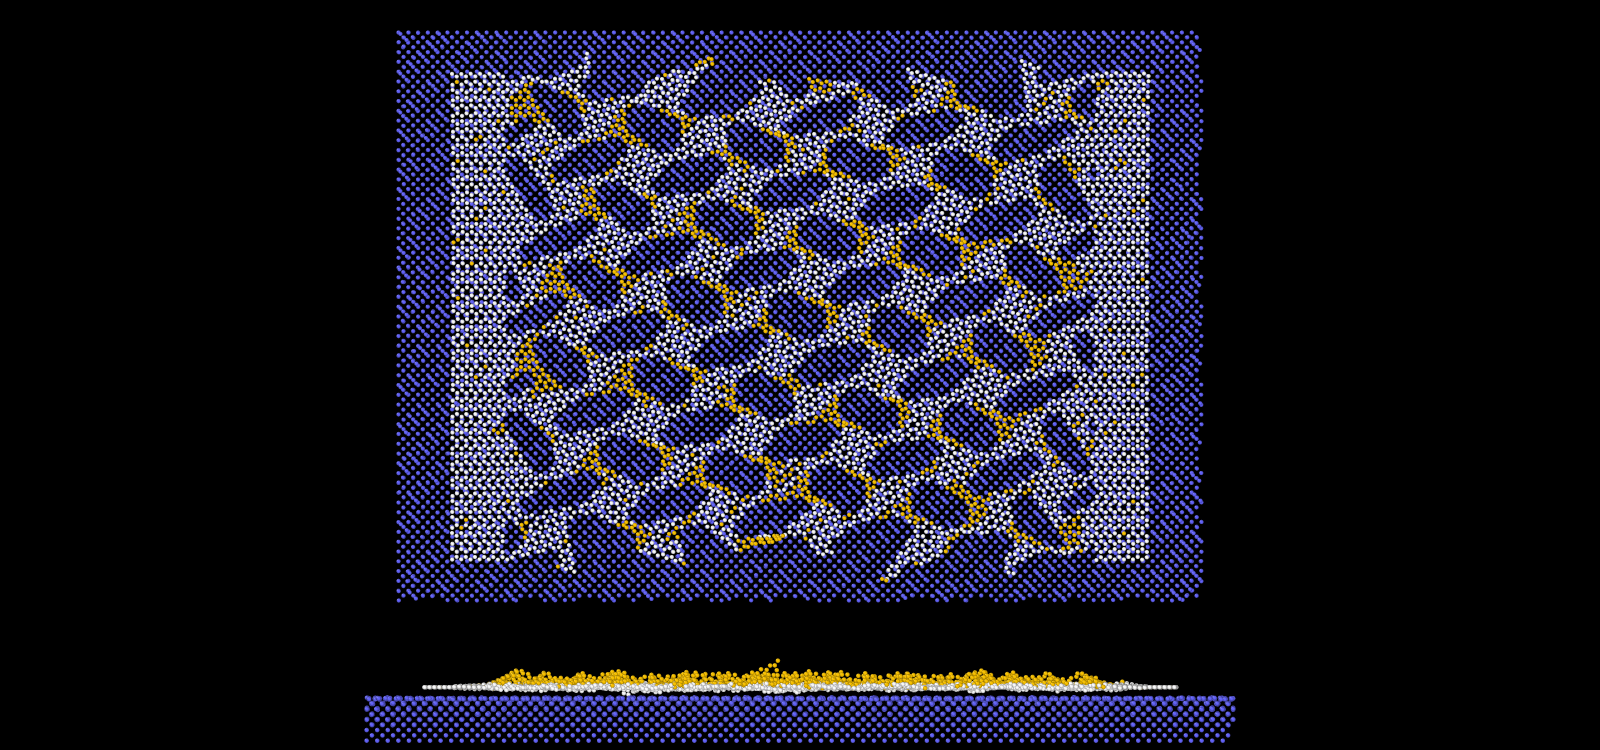
\includegraphics[width=\textwidth]{figures/baseline/contact_vs_stretch/popup/pop_stretch0020.png}
        \caption{Strain = 0.20}
        % \label{fig:}
    \end{subfigure}
    \begin{subfigure}[b]{0.49\textwidth}
        \centering
        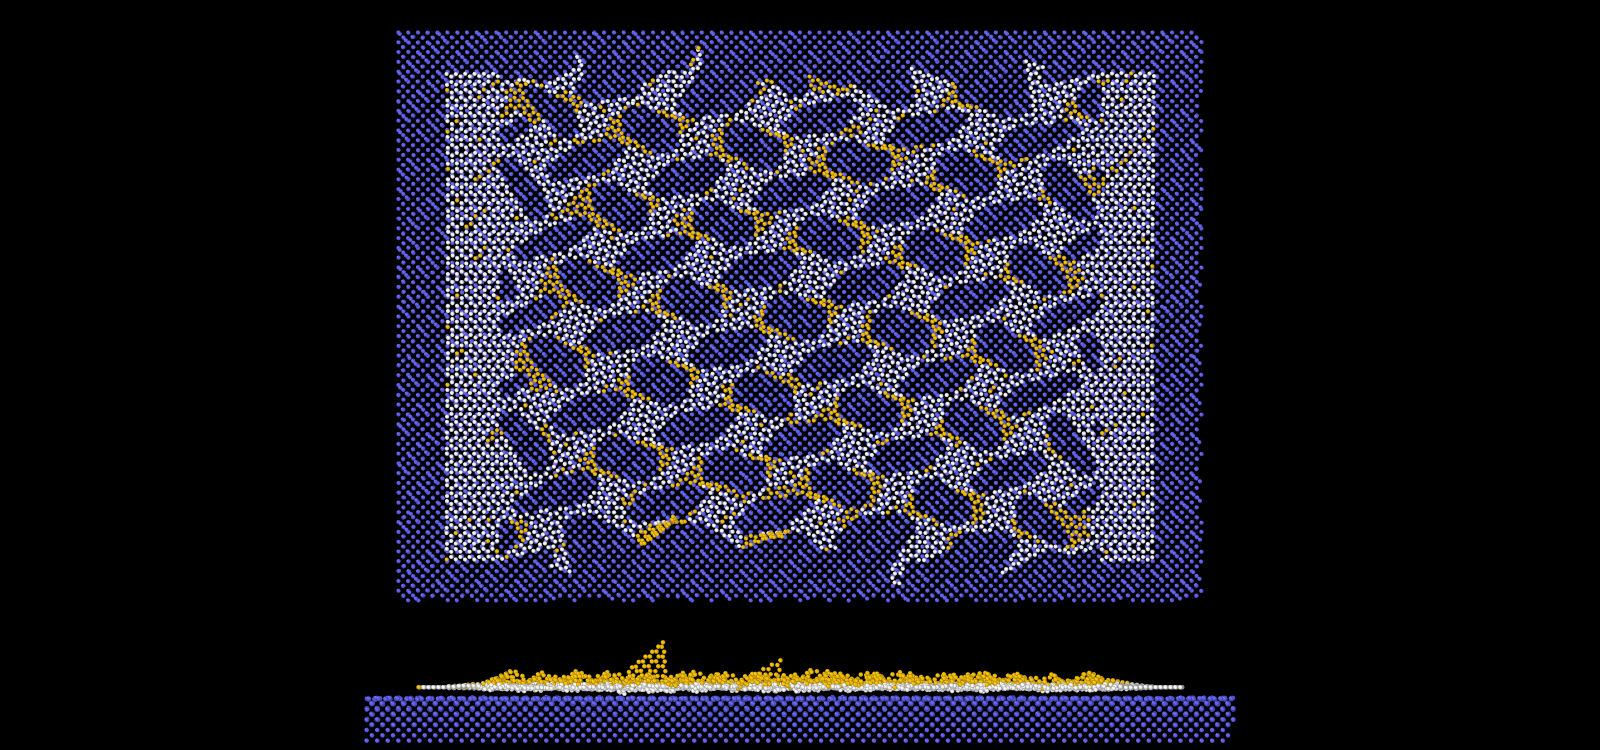
\includegraphics[width=\textwidth]{figures/baseline/contact_vs_stretch/popup/pop_stretch0022.png}
        \caption{Strain = 0.22}
        \label{fig:tetrahedron_strain_j}
    \end{subfigure}
    \hfill
       \caption{Straining of the Tetrahedron $(7,5,1)$ pattern against substrate. The top part of each frame (a)-(j) shows a top-down view into the x-y plane, with the y-direction on the horizontal axis and the x-direction on the vertical axis. The bottom part of each frame shows a side-view of the system, the y-direction on the horizontal axis and the z-direction on the vertical axis. White-colored atoms indicate graphene sheet atoms in contact with the substrate while the yellow-colored atoms are not in contact.}
       \label{fig:tetrahedron_strain}
  \end{figure}

% Honeycomb (contact)
\begin{figure}[H]
    \centering
    \begin{subfigure}[b]{0.49\textwidth}
        \centering
        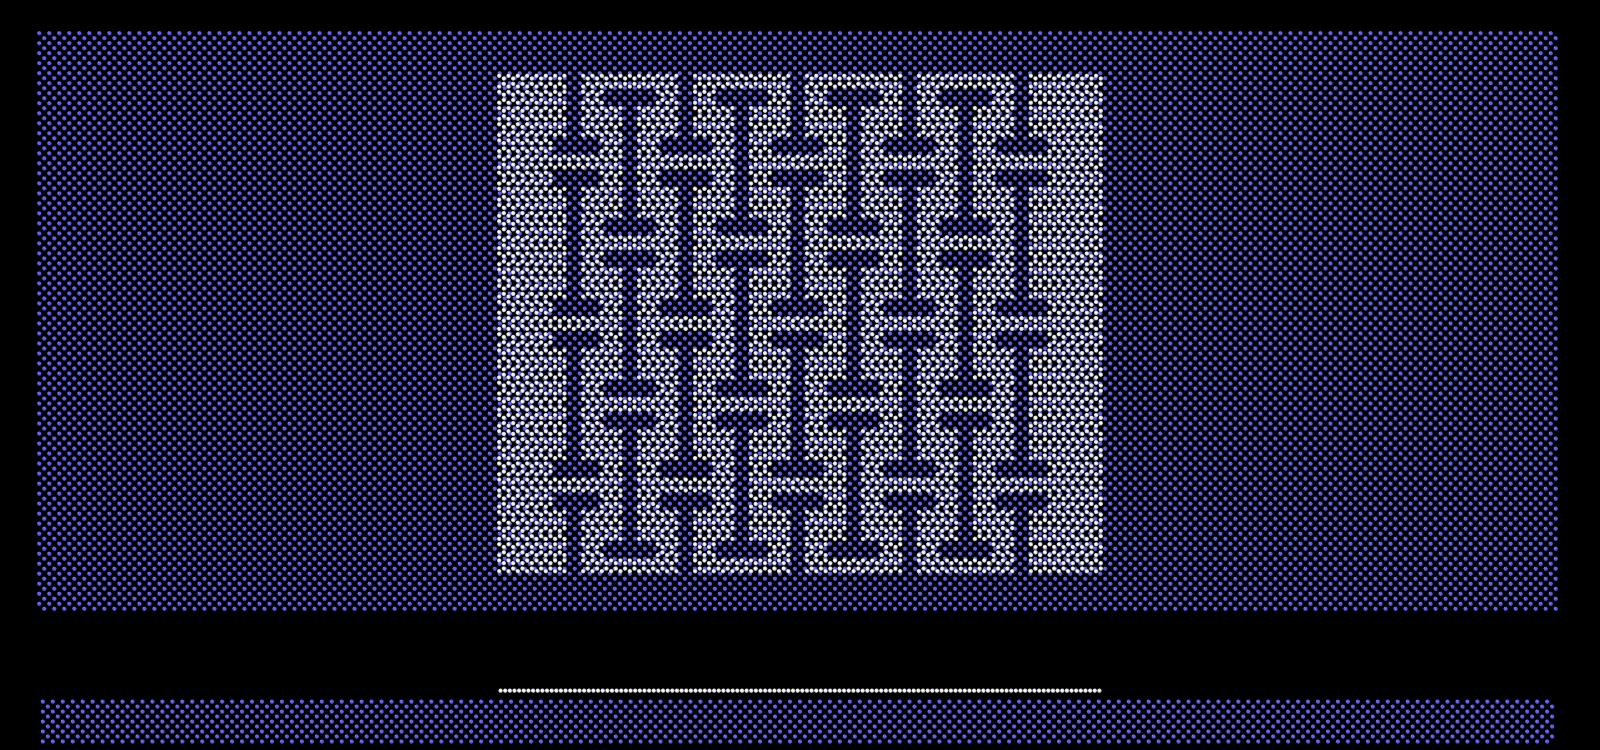
\includegraphics[width=\textwidth]{figures/baseline/contact_vs_stretch/honeycomb/hon_stretch0000.png}
        \caption{Strain = 0.00}
        % \label{fig:}
    \end{subfigure}
    \hfill
    \begin{subfigure}[b]{0.49\textwidth}
        \centering
        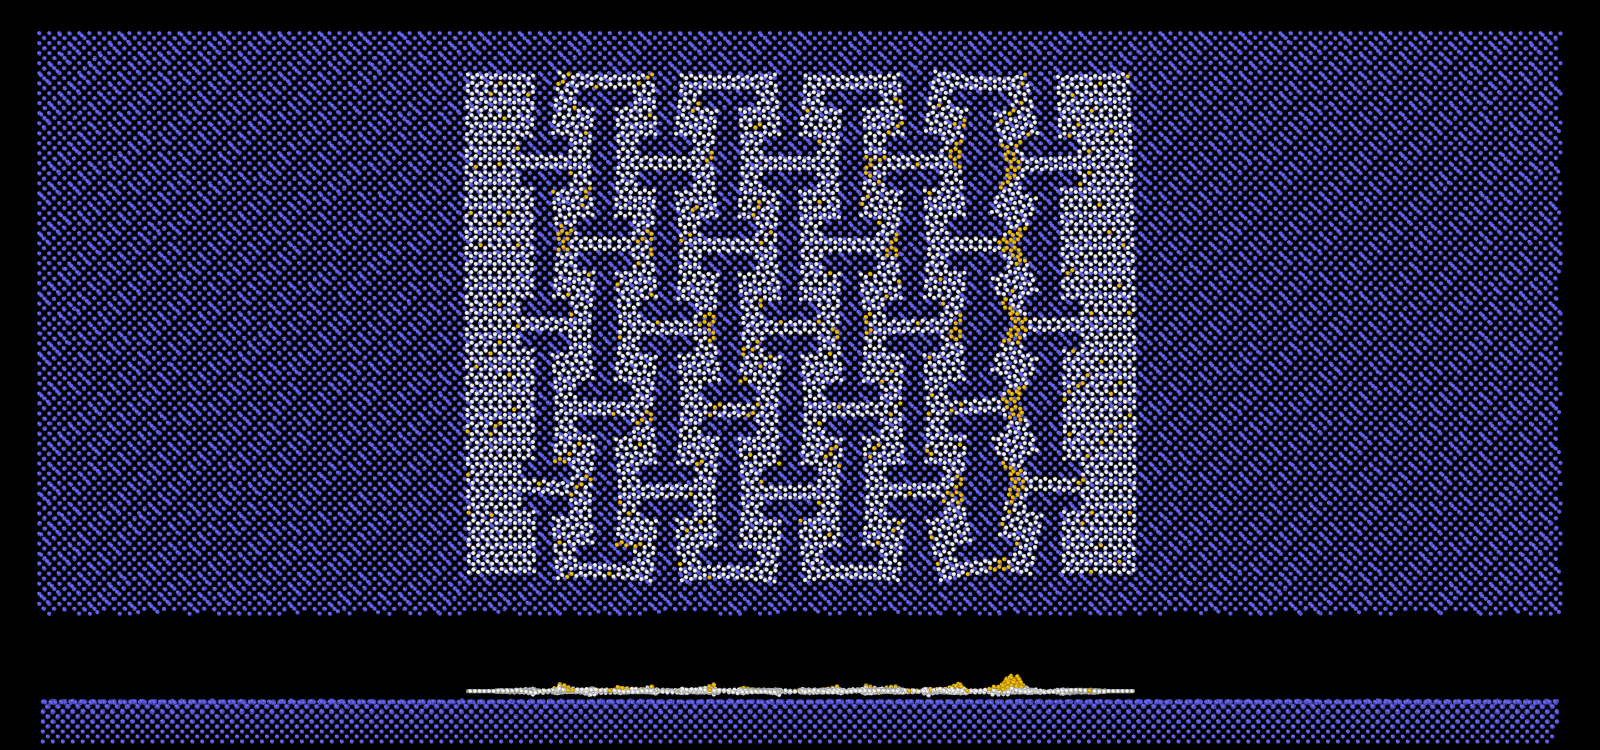
\includegraphics[width=\textwidth]{figures/baseline/contact_vs_stretch/honeycomb/hon_stretch0014.png}
        \caption{Strain = 0.14}
        % \label{fig:}
    \end{subfigure}
    \begin{subfigure}[b]{0.49\textwidth}
        \centering
        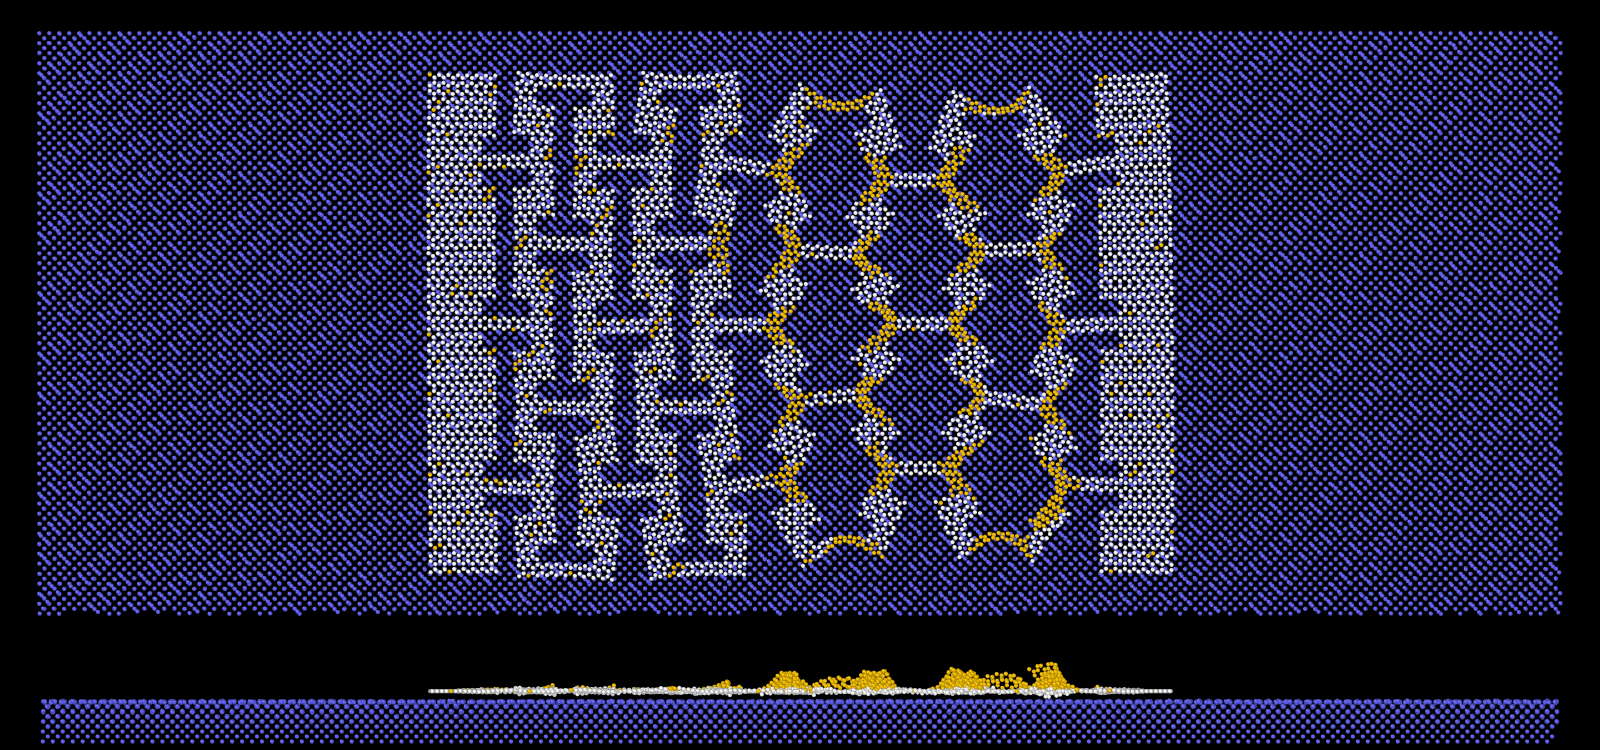
\includegraphics[width=\textwidth]{figures/baseline/contact_vs_stretch/honeycomb/hon_stretch0028.png}
        \caption{Strain = 0.28}
        % \label{fig:}
    \end{subfigure}
    \hfill
    \begin{subfigure}[b]{0.49\textwidth}
        \centering
        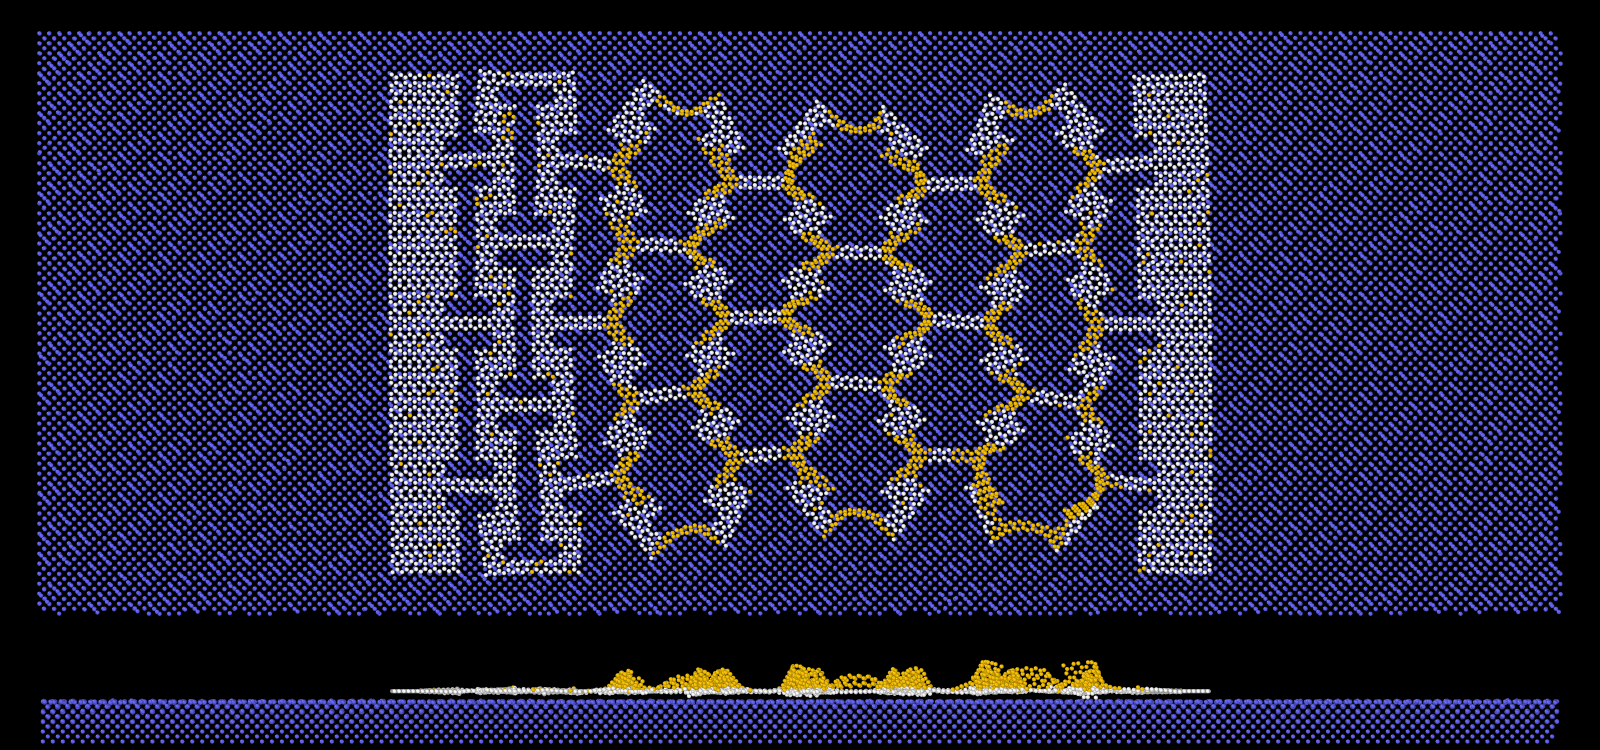
\includegraphics[width=\textwidth]{figures/baseline/contact_vs_stretch/honeycomb/hon_stretch0042.png}
        \caption{Strain = 0.42}
        % \label{fig:}
    \end{subfigure}
    \hfill
    \begin{subfigure}[b]{0.49\textwidth}
        \centering
        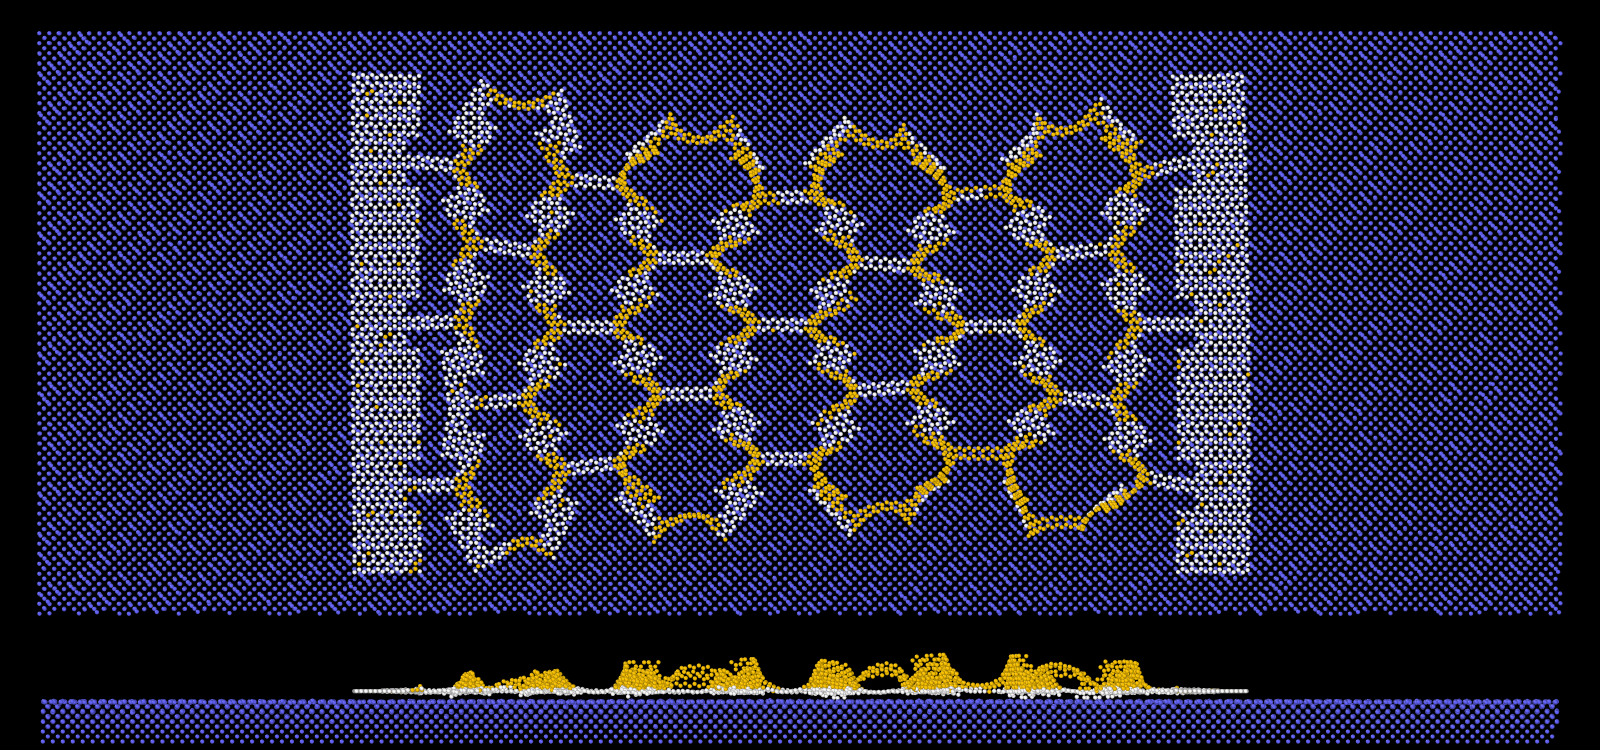
\includegraphics[width=\textwidth]{figures/baseline/contact_vs_stretch/honeycomb/hon_stretch0056.png}
        \caption{Strain = 0.56}
        % \label{fig:}
    \end{subfigure}
    \hfill
    \begin{subfigure}[b]{0.49\textwidth}
        \centering
        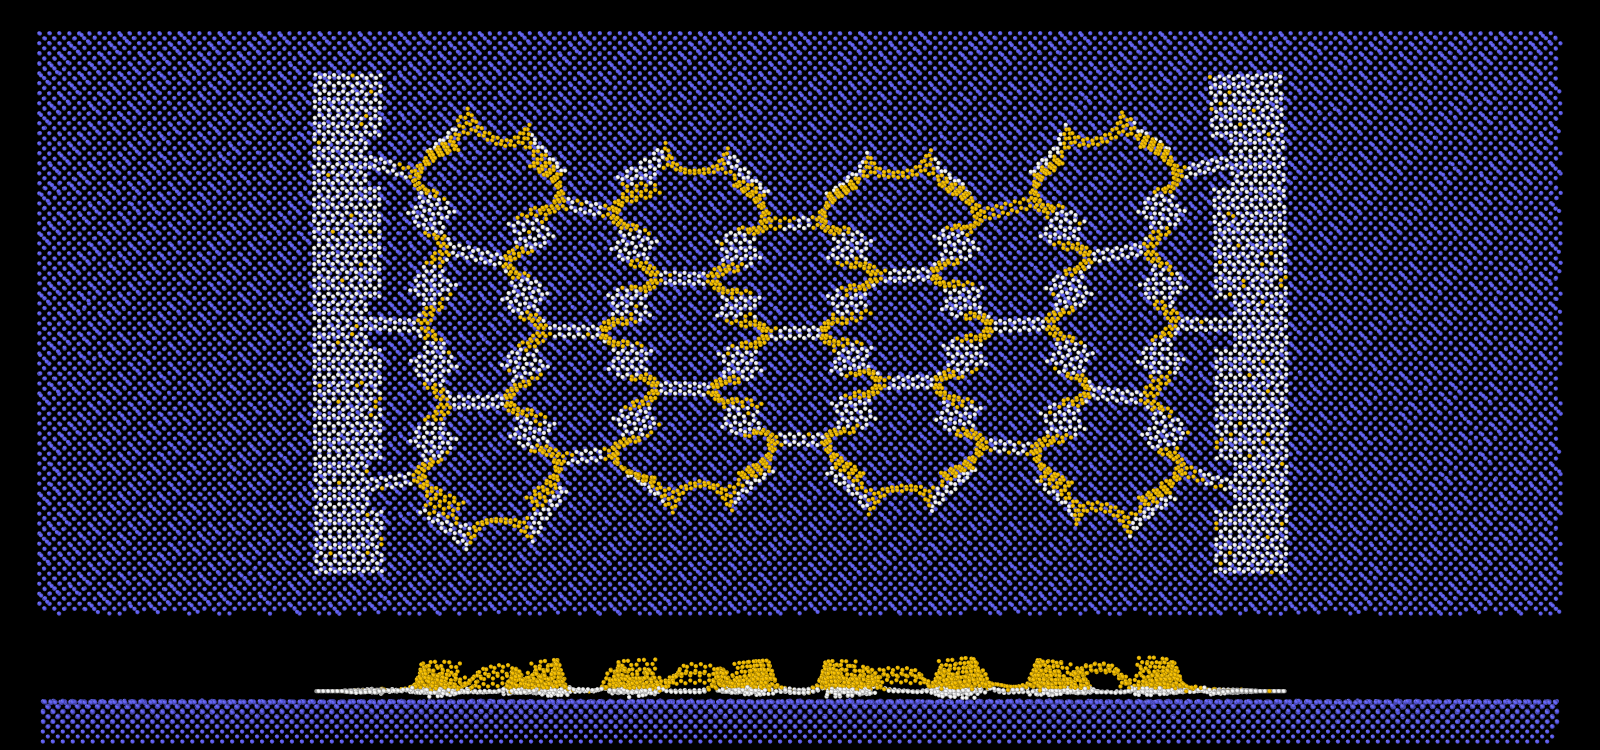
\includegraphics[width=\textwidth]{figures/baseline/contact_vs_stretch/honeycomb/hon_stretch0070.png}
        \caption{Strain = 0.70}
        % \label{fig:}
    \end{subfigure}
    \begin{subfigure}[b]{0.49\textwidth}
        \centering
        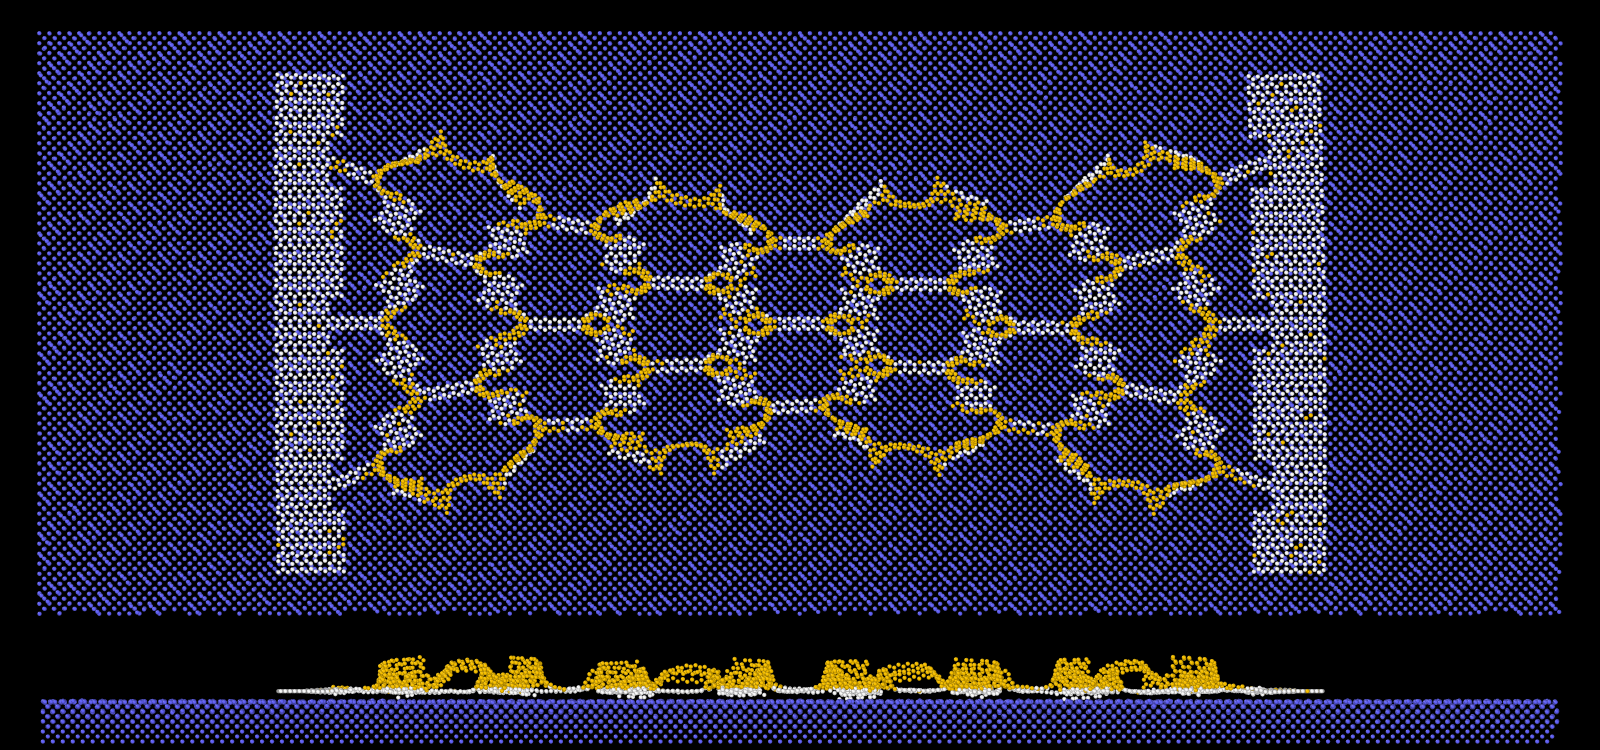
\includegraphics[width=\textwidth]{figures/baseline/contact_vs_stretch/honeycomb/hon_stretch0084.png}
        \caption{Strain = 0.84}
        % \label{fig:}
    \end{subfigure}
    \hfill
    \begin{subfigure}[b]{0.49\textwidth}
        \centering
        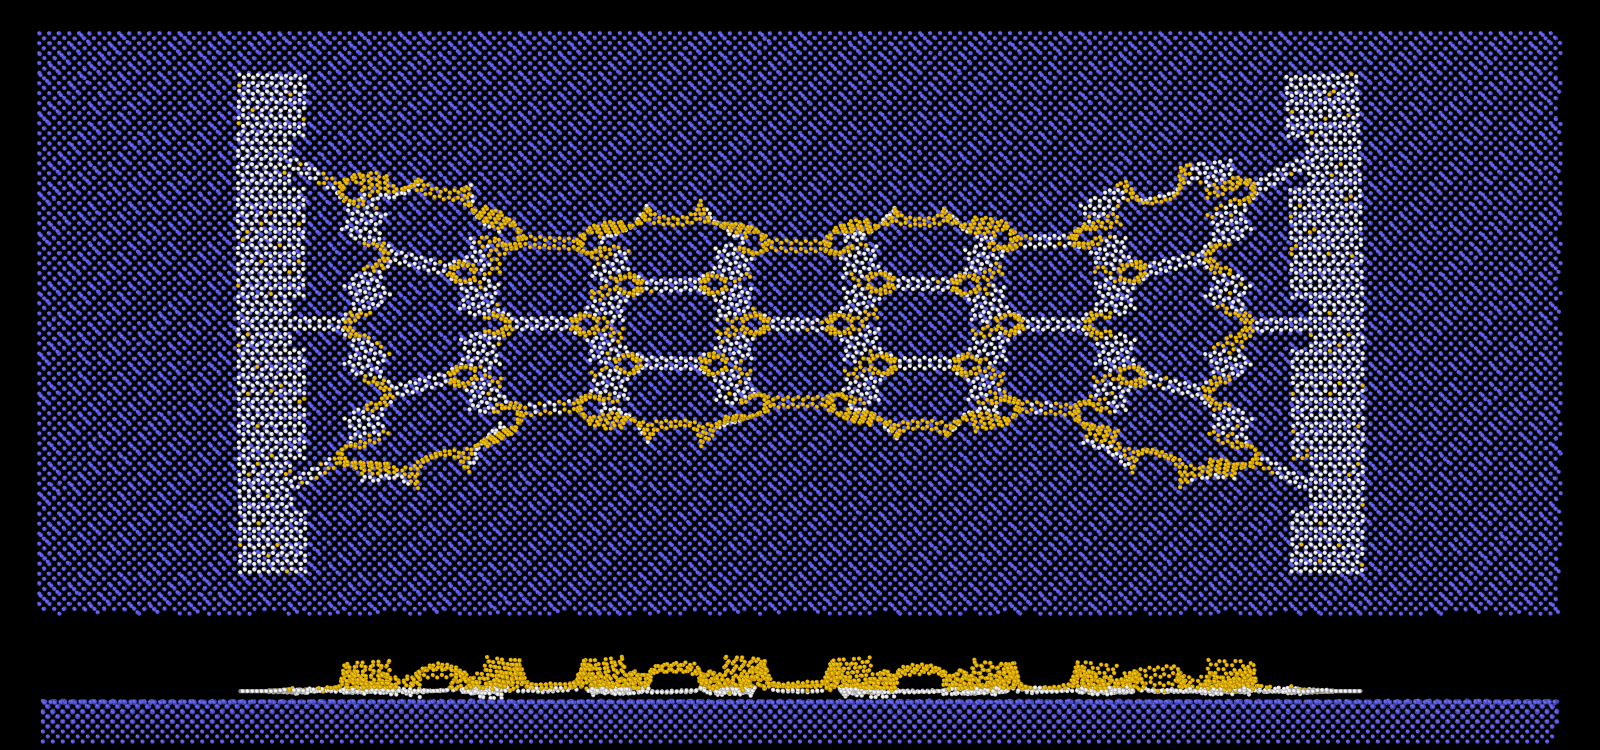
\includegraphics[width=\textwidth]{figures/baseline/contact_vs_stretch/honeycomb/hon_stretch0098.png}
        \caption{Strain = 0.98}
        % \label{fig:}
    \end{subfigure}
    \begin{subfigure}[b]{0.49\textwidth}
        \centering
        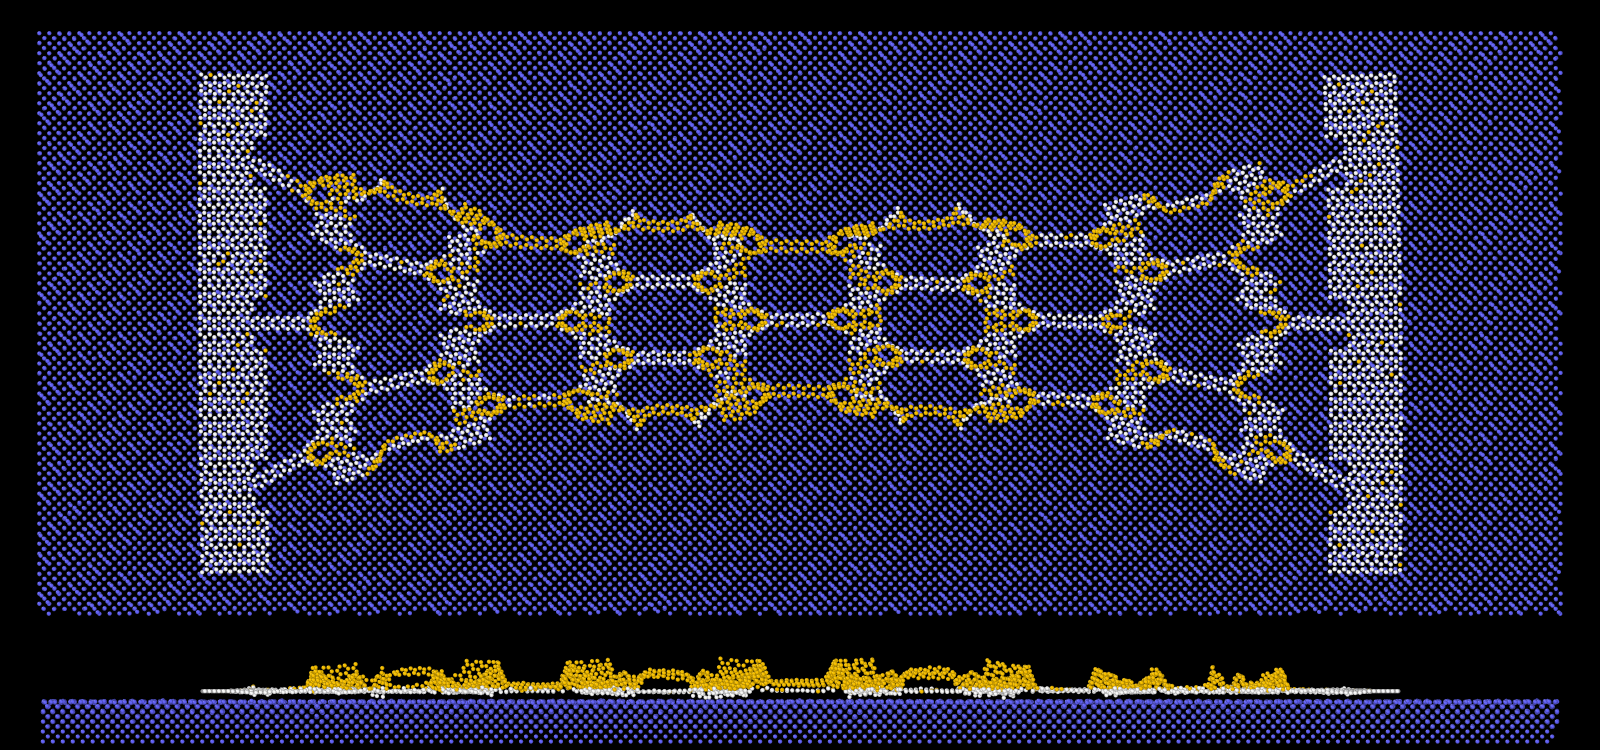
\includegraphics[width=\textwidth]{figures/baseline/contact_vs_stretch/honeycomb/hon_stretch0112.png}
        \caption{Strain = 1.12}
        % \label{fig:}
    \end{subfigure}
    \begin{subfigure}[b]{0.49\textwidth}
        \centering
        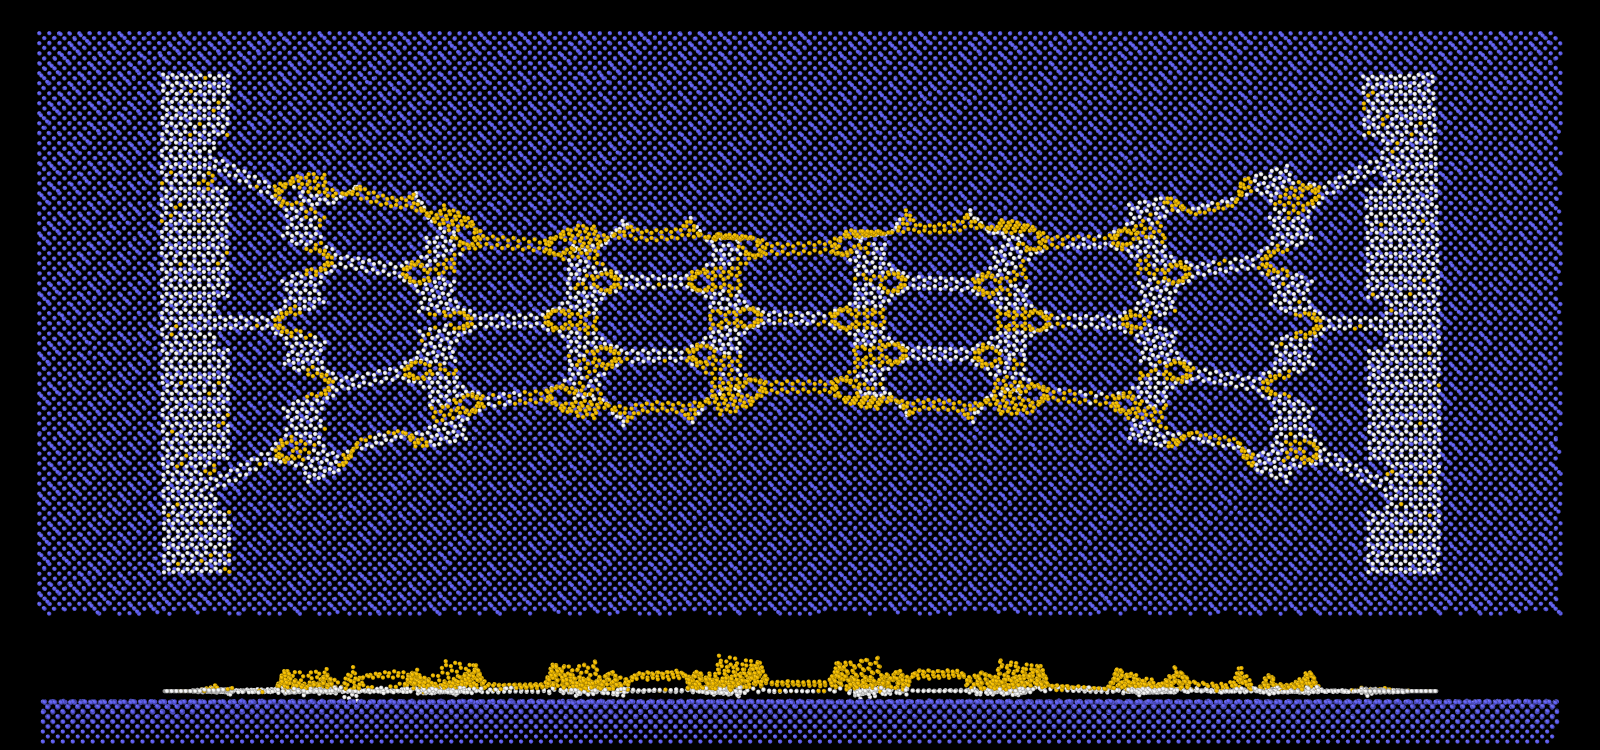
\includegraphics[width=\textwidth]{figures/baseline/contact_vs_stretch/honeycomb/hon_stretch0126.png}
        \caption{Strain = 1.26}
        % \label{fig:}
    \end{subfigure}
    \hfill
       \caption{Straining of the Honeycomb $(2,2,1,5)$ pattern against substrate. The top part of each frame (a)-(j) shows a top-down view into the x-y plane, with the y-direction on the horizontal axis and the x-direction on the vertical axis. The bottom part of each frame shows a side-view of the system, the y-direction on the horizontal axis and the z-direction on the vertical axis. White-colored atoms indicate graphene sheet atoms in contact with the substrate while the yellow-colored atoms are not in contact.}
       \label{fig:honeycomb_strain}
  \end{figure}
  



  

